\chapter{Chapter Name} \label{chap:intro}
\graphicspath{{../figs/}} 

%******************************************************************************************************************************************************


%+++++++++++++++++++++++++++++++++++++++++++++++++++++++++++++++++++++++++++++++++++++++++++++++++++++++++++++
\section{Section 1} \label{sec:sec1}

You can reference a Section \ref{sec:sec1} or Subsction
\ref{sec:subsec} in that way. 
You can also cite some bibliogrhapic stuff \citep{ExArt01,ExIncollec01,ExInpro01,ExTech01,ExBook01,ExPHD01}.
In here we reference the Figure~\ref{fig:fig1}.
And also the table

\begin{figure}[!b]	
	\begin{center}
		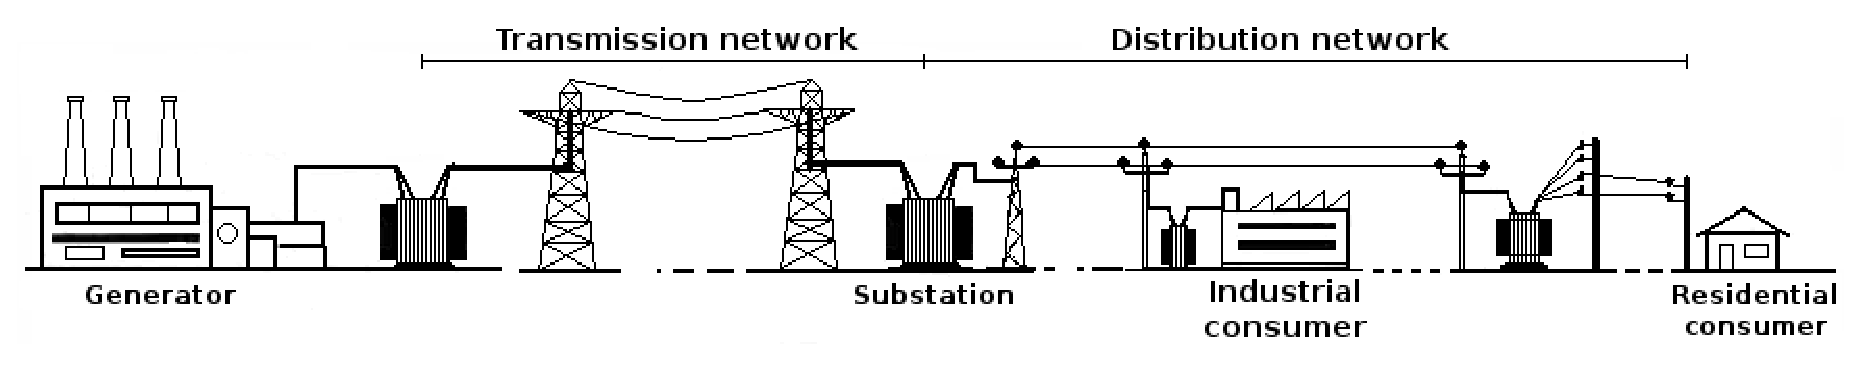
\includegraphics[width=0.95\textwidth]{grid_sketch.eps} \\ 
		\caption[Short description for the index.]
		{Caption under the figures.}		
		\label{fig:fig1}	
	\end{center}
\end{figure}


%--------------------------------------------------------------------------------------------------------------
\subsection{Subsection}
\label{sec:subsec}

We can also reference an Equation \ref{eq:ctrnn}.
\begin{equation}
\begin{array}{l}
\dot y_{i}(t)= f_i(y_1(t),y_2(t)) = \\ 
= \frac{1}{\tau_i}\cdot\left(-y_i(t)+\sum_{j=1}^2w_{ij}\cdot \varphi\left(y_j(t)+\theta_j\right)+x_i(t)\right) \\\\
with\;\varphi(x)=\frac{1}{1+e^{-x}}\;\;and\;\;i=1,2.
\end{array}
\label{eq:ctrnn}
\end{equation}

Make a list of items
\begin{itemize}
\item{{\it Item 1}:}
Description.
\item{{\it Item 2}:}
Description \footnote{
This is a footnote.
}.
\end{itemize}

Or even a Table \ref{tab:table1}

\begin{table}[!t]
  \centering
  \resizebox{0.75\textwidth}{!}{%
  \begin{tabular}{lcc} \toprule
    \multirow{2}{*}{Appliance} & Consumption & Share of total \\ 
                               & (Wh/day)    & (\%)           \\ \midrule
    \multicolumn{3}{l}{\emph{Deferrable}}                     \\
    Washing machine            & 785.92      & 6.95           \\ 
    Dryer                      & 962.6       & 8.5            \\
    Dishwasher                 & 693.6       & 6.13           \\
    Total (deferrable)         & 2442.12     & 21.6           \\ \midrule
    \multicolumn{3}{l}{\emph{Non-deferrable}}                 \\
    Lights                     & 1302        & 11.5           \\
    Oven                       & 1255.15     & 11.1           \\
    Fridge                     & 616.73      & 5.4            \\
    Computers and              &             &                \\
    entertainment              & 5694        & 50.03          \\  
    appliances (TV,DVD,etc.)   &             &                \\
    Total (Non-deferrable)     & 8867.88     & 78.4           \\ \midrule
    Total                      & 11310       & 100            \\ \bottomrule
  \end{tabular}}
  \caption[Short description of the table.]
  {Caption under the table.}
  \label{tab:table1}
\end{table}


